\section{State of the art}
\label{stateart}
%

%
Display used for common Head Mounted Display (HMD) are 
various, we try to explain the chief differences. In the
following we will examine five types: LCD, AMLCD, LCOS, 
FLCOS, OLED.
%

%
\subsection{LCD}
The LCD technology is based on the light modulating properties 
of liquid crystals (LCs). Since LCs are not able to emit light 
directly, actual LCD panels and displays need a light source.
%
That is why such devices are often classified as "passive" 
displays. 
%
LCD displays are usually for a general purpose use, but they 
can also be tuned for a specific usage - e.g. the displaying 
of highly detailed still images or of highly dynamic, 
fast-changing video content.
%
Because of their versatility, they are used in a wide range 
of applications including computer monitors, TVs, aircraft 
cockpits. They're also common in electronic consumer devices 
such as video player, gaming devices, etc.
%
Compared to other display-making technologies - such as CRT - 
LCD allows to make wider and flatter displays while reducing 
electrical power consumption and, thus, making LCD displays 
also well-suitable for mobile devices.
%

%
\subsection{AMLCD}
Active Matrix LCDs (AMLCD) use a matrix of thin-film transistors 
(TFTs) to achieve better performance compared to normal LCD screens. 
They still have polarizing sheets and cells of liquid crystal 
(same as LCD), but the TFTs allow to store the electrical state 
of each pixel on the display while all the other pixels are 
being updated.
%
The advantages of a TFT-LCD monitor are many. It provides a 
larger viewing-angle and a much brighter display than a passive 
matrix monitor with the same size. Some designs have replaced 
transistors with other components such as diodes.
%
With an active matrix only the desired pixel receives a charge, 
acting as a capacitor and holding the charge until the next refresh 
cycle (transistors have the ability to hold a charge for a limited 
period of time). On the contrary, a passive matrix display delivers 
current to the liquid crystals in a specific area with a simple 
conductive grid. AMLCD can be more accurate because, thanks to 
the switching action of transistors, only a the specific pixels 
receive a charge, improving image quality with respect to a 
passive matrix display.
%
AMLCDs are most popular type of display on the market today.

\subsection{LCOS}
Liquid crystal on silicon (LCOS) is a {\it micro-projection} or 
{\it micro-display} technology typically applied in projection 
televisions. It is a reflective technology and uses liquid crystals.
%
LCoS displays are well-suited for high resolution and high contrast 
images. 
%
There are two broad categories of LCoS displays: three-panel and 
single-panel. In three-panel designs, there is one display chip 
per color, and the images are combined optically. Single-panel 
designs, instead, makes use of only one display chip  that shows 
the red, green, and blue components in succession with the 
observer's eyes relied upon to combine the color stream. 
%
If the frequency of the color fields is lower than about 540 Hz, 
an effect called "color breakup" is seen, where false colors 
are briefly perceived when either the image or the observer's 
eye is in motion.
%

%
\subsection{FLCOS}
FLCOS devices are made using ferroelectric liquid crystals 
(so the technology is named FLCoS), which are inherently faster 
than other types of liquid crystals.
%

%
\subsection{OLED}
The Organic Light Emitting Diode (OLED) takes advantage of an 
electroluminescent layer, made of organic compounds, used 
like a LED. This layer is wrapped between two electrodes and 
at least one of the electrodes is transparent.
%
OLEDs are a young display technology, not yet able to emit as 
much light per unit area as an inorganic solid-state based LED. 
For this reason OLED are not used as point-light sources.
%
This devices can be used for multiple applications, from 
television and computer screens to small and portable system 
screens such as mobile phones, PDAs and head-mounted displays 
(where high-resolution is needed).
%
Since OLED displays do not require a backlight, they can 
perform deep black levels and be thinner and lighter than 
LCD panels. Besides, OLED displays can achieve higher contrast 
ratios. Even the power drain is lower, compared to LCD screen.
%

%
\subsection{A comparison towards displays}
By using AMLCD display for Head Mounted Display (HMD) the entire 
device is more compact, because AMLCDs only need a flat backlit 
panel rather than a complex (and thicker) illumination unit. 
This is the reason why FLCOS and LCOS displays are commonly not used. 
%
On the other hand, AMLCD display has relatively low contrast ratio 
and provides the lowest luminance range and largest pixel dimensions 
among all of the previously seen technologies.
As well as AMLCD, OLED offer a compact system design due to its 
self-emission nature. In addition, OLEDs provide a good range of 
luminance, even tough the resolution and contrast ratio of 
existing OLEDs are relatively low compared with FLCOS and LCOS microdisplays.
%
Besides, OLEDs life span would be shortened if the display 
luminance is high (e.g. more than 100 cd/m2).
%
According to \cite{Zhang:08}, for HMD designs a display panel around 2.50 cm is 
preferable as it would offer a good balance of compactness and the 
focal length range of the optics. In fact, when dealing with small 
display panels, shorter focal length and larger magnification are 
required in order to achieve a reasonable field-of-view (FOV). 
%
LCOS microdisplays offer the highest resolution and contrast compared 
with other types of displays and they are commonly used as image 
sources in digital projectors. 
%

%
\begin{figure}[!h]
  \begin{center}
    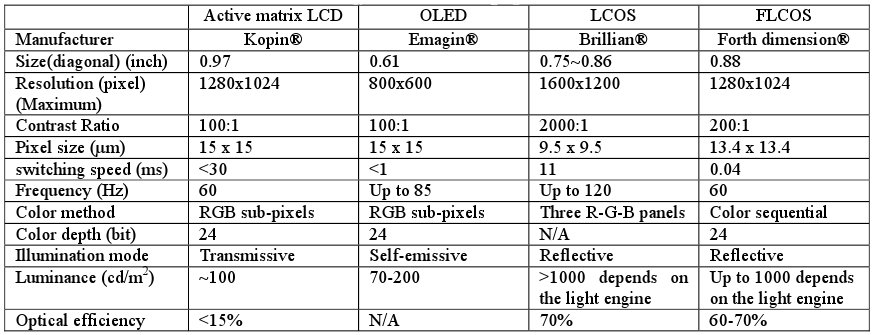
\includegraphics[width=400pt]{img/hmd_comparison_table}  %logo
  \end{center}
\end{figure}
%

%
The liquid crystal used in LCOS microdisplays, however, has low 
switching speed, which makes it impossible to use color sequential 
method, to achieve a full color mode. FLCOS offers high pixel 
resolution, luminance output, image contrast, and optical efficiency. 
Also, the fast response speed of ferroelectric liquid crystal makes 
it possible to achieve full-color display using a single-panel color 
sequential scheme. On the other hand, it requires a carefully designed 
illumination unit to achieve high contrast and high luminance, which 
makes the overall display system less compact than a system using 
AMLCD or OLED microdisplays.
